\documentclass[a4paper,11pt]{article}
\usepackage{a4wide,graphicx,amssymb, amstext, amsmath, epstopdf, booktabs, verbatim, geometry, appendix, natbib, lmodern, tabularx, enumitem, longtable, hyperref, subcaption}

%\geometry{letterpaper}
%\usepackage{garamond}

\newcommand*\Title{Trafic Control System}
\newcommand*\cpiType{Software Design Document}
\newcommand*\Author{}
\title{\Title}
\author{}
\date{\today}
%-----------------------------------------------------------

\usepackage{template/template} % This is what makes your document look like a cpi document.


\begin{document}

\begin{titlepage}
\maketitle
\end{titlepage}

  	\linespread{1.15} %Set standard document linespacing
    
  	\subsection*{Background and Context}
  	This software design document provides details and decisions made for building the "Traffic control system" application. For this a graphical representation UML is used including class diagrams and sequence diagrams.
  	
  	\subsection*{Definitions and abreviations}
  	\begin{longtable}[l]{p{80pt} p{350pt}} 
  		UML & Unified Modeling Language\\
  		MVVM & Model view viewmodel\\
  	\end{longtable}
  	
  	\tableofcontents
 
  	\newpage
  	
  	\section{System overview}
\begin{figure}[!ht]
	\centering
	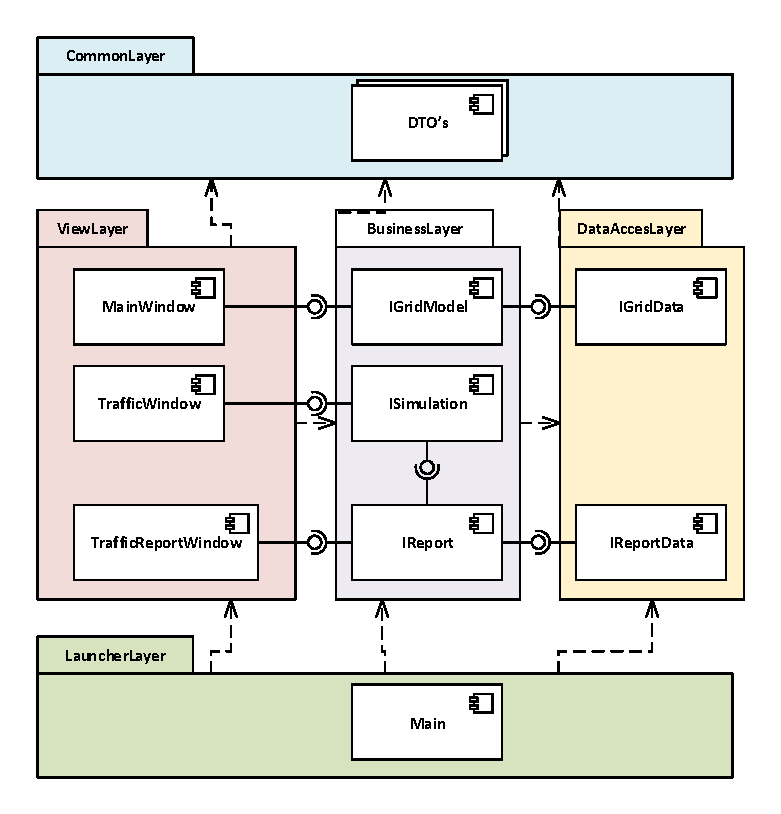
\includegraphics[width=0.8\textwidth]{figures/architecture}
	\caption{System overview}
	\label{fig:sys}
\end{figure}

\subsection{Abstraction layers}
We design the software according to SOLID principles, which are common rules used for the design of the software. The classes should have only one responsibility, hence our representation logic and business logic are separated. We also use an interface driven design combined with the dependency inversion principle, hence we handle dependencies using dependency injection. By following these rules the system is more testable and abstracted. 

\subsubsection{Common layer}
The \texttt{CommonLayer} can be accessed by any layer, and the layer only contains DTO's. Important about the classes of the \texttt{CommonLayer} is that they contain no logic at all, hence they only have data. The purpose for this is for easy serialization and a easy way to pass the data through all the layers.

\subsection{View layer}
Inside of the \texttt{ViewLayer} is al the representation logic, this layer handles showing an user interface. For the representation the \texttt{MVVM} model is used, this pattern keeps the design and the code of the view seperate.

\subsection{Business Layer}
This layer contains the business logic of the system, it makes sure that all the business rules are followed. Hence this is the brain of the application which is allowed to make changes to the DTO's from the \texttt{CommonLayer}.

\subsection{Data Layer}
The data layer contains the logic for serializing the objects from the \texttt{Common Layer} to another storage. For this application the objects will be serialized to a file.

\subsection{Other layers}
The application has tests and it also require a launcher layer. Because the application can not be launched from the \texttt{ViewLayer} since it has no reference to the \texttt{DataAccesLayer}. So in the launcher layer all the dependencies will be handled. 
  	\section{Class diagrams}


  	\section{Sequence diagrams}
\begin{figure}[!ht]
	\centering
	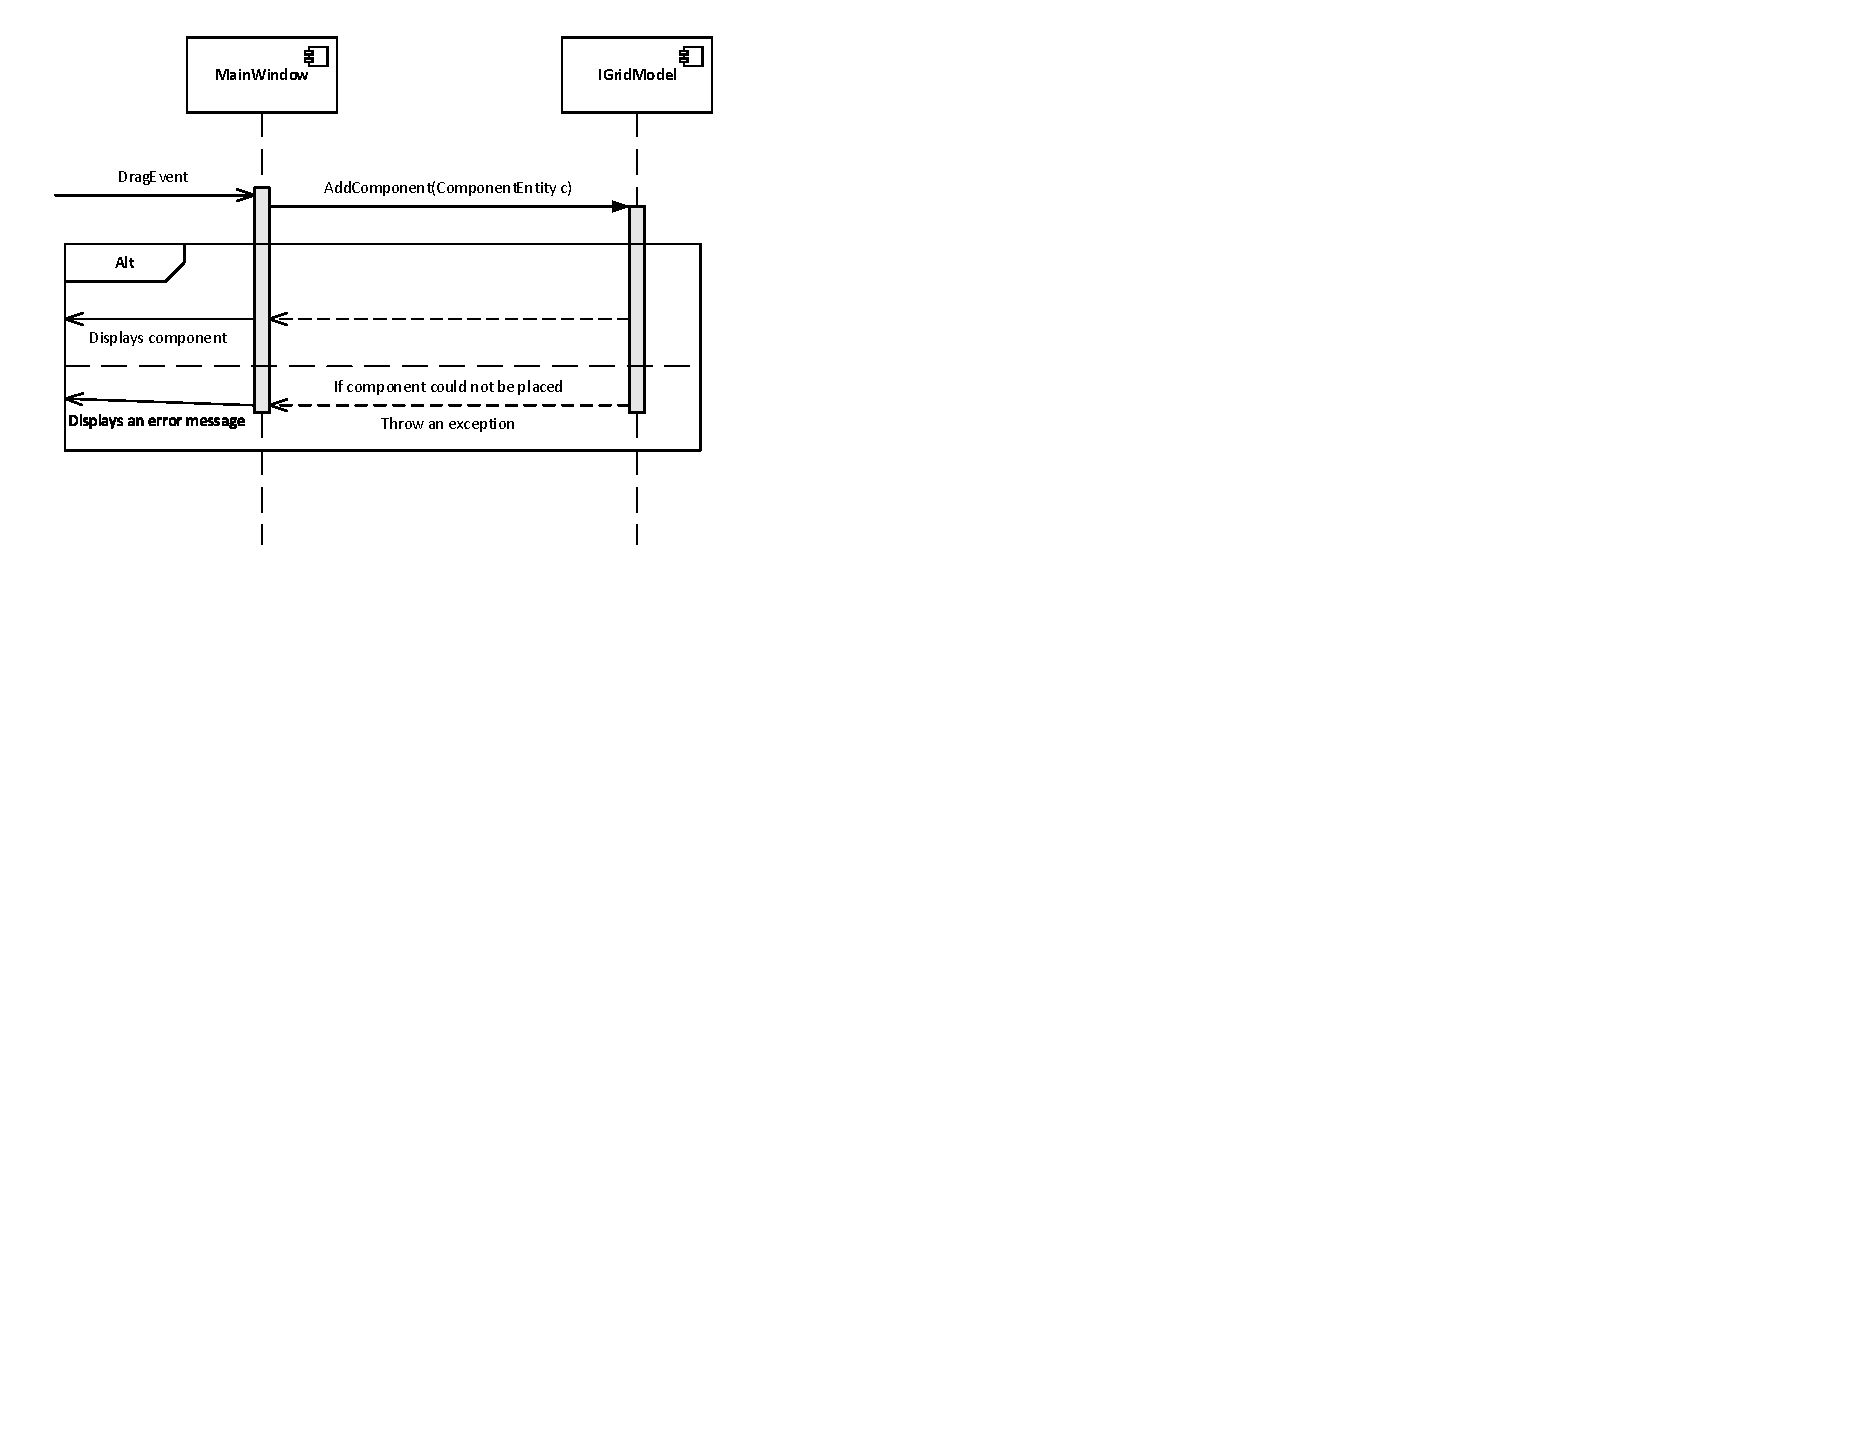
\includegraphics{figures/PosititioningCrossroad}
	\caption{Positioning crossroad.}
\end{figure}

\begin{figure}[!ht]
	\centering
	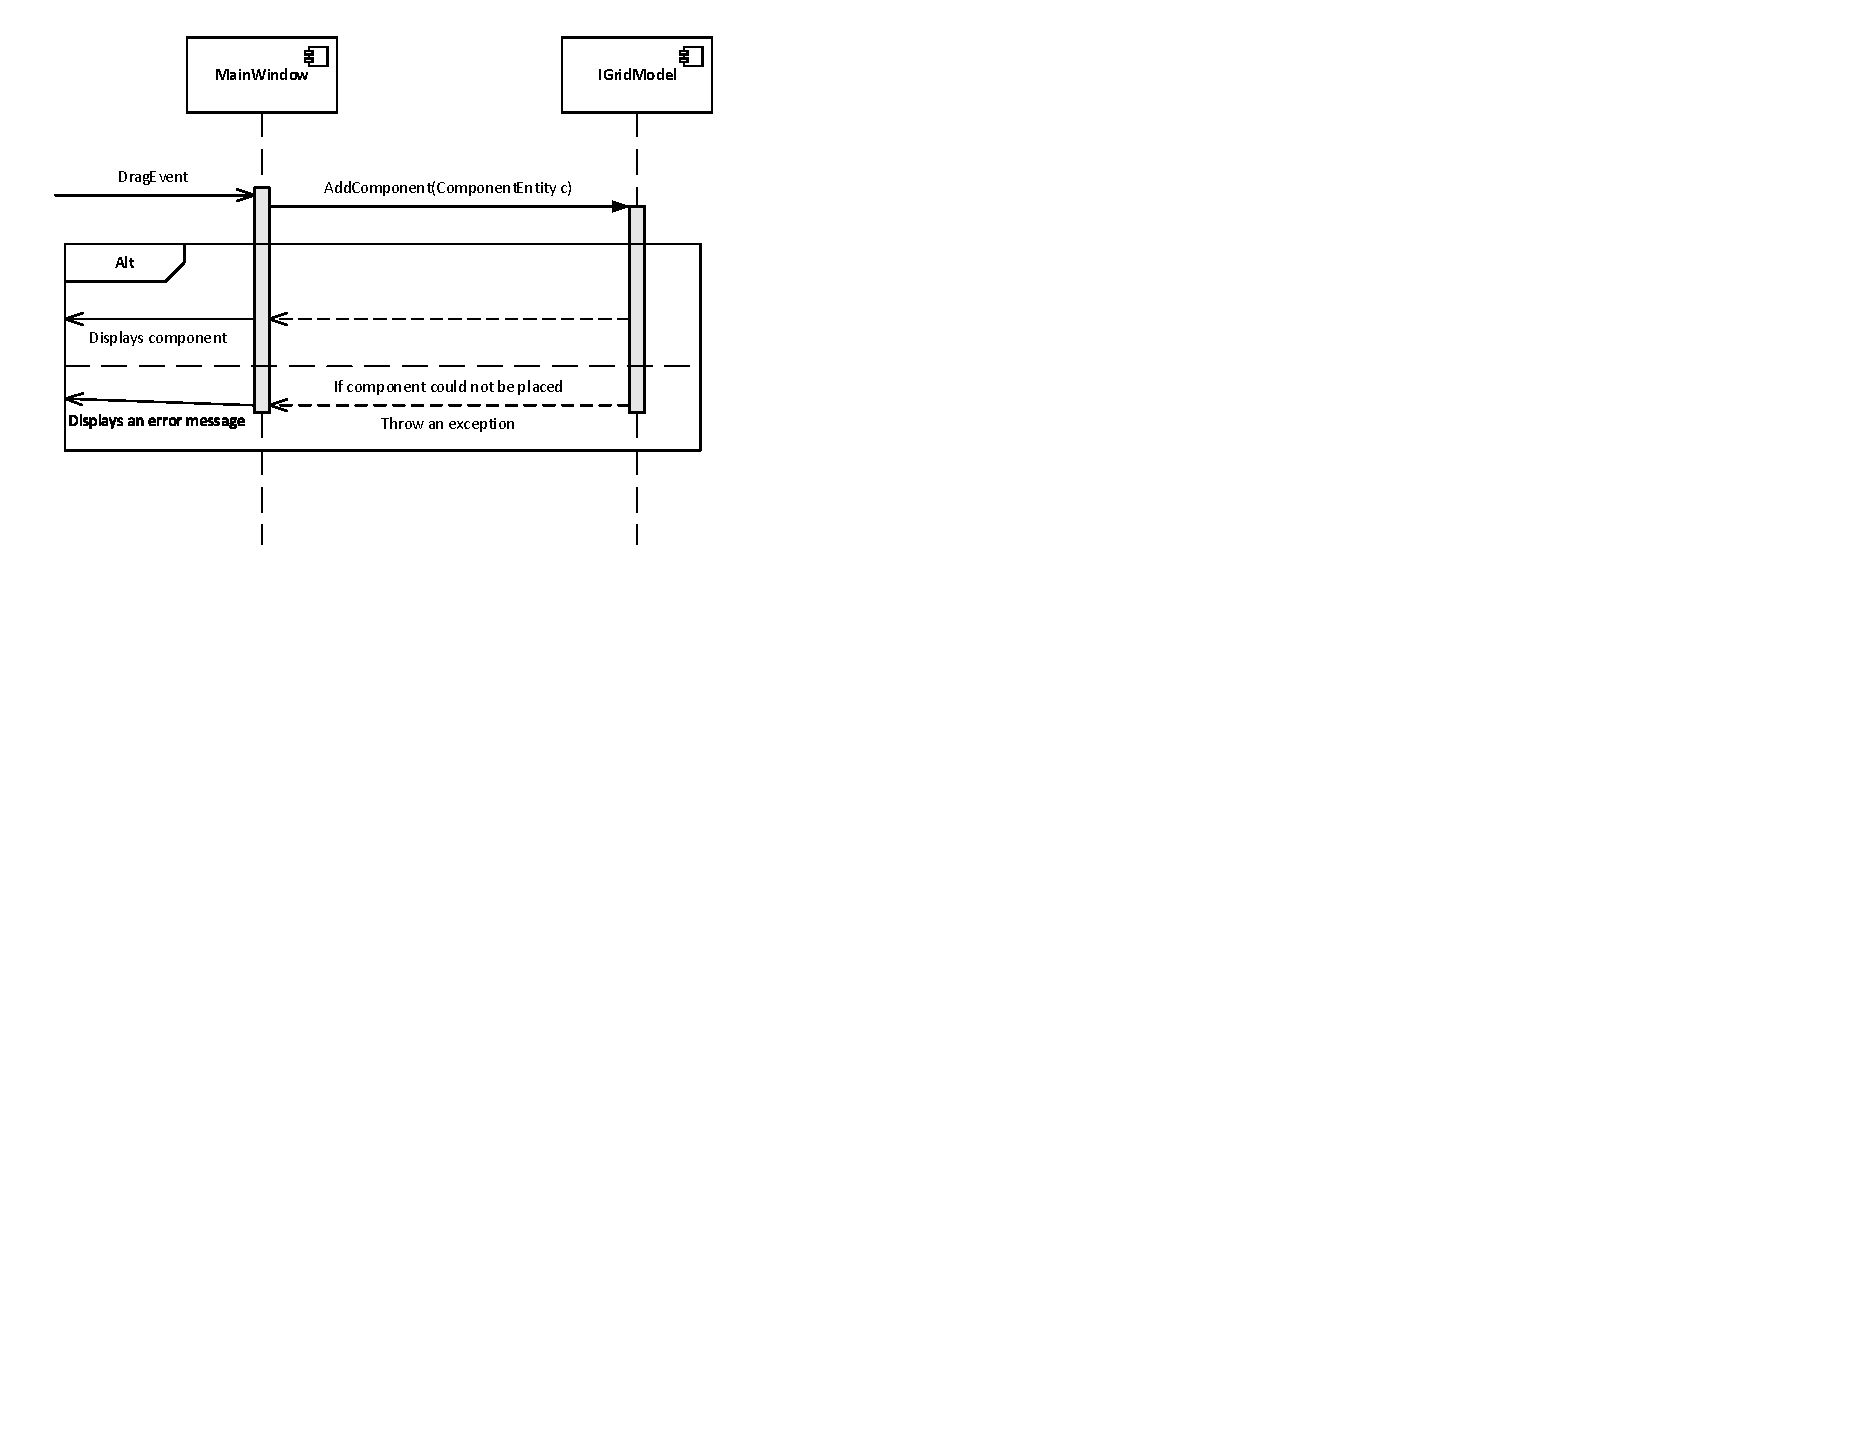
\includegraphics{figures/ConfigTrafficLight}
	\caption{Configuring traffic light times.}
\end{figure}

\begin{figure}[!ht]
	\centering
	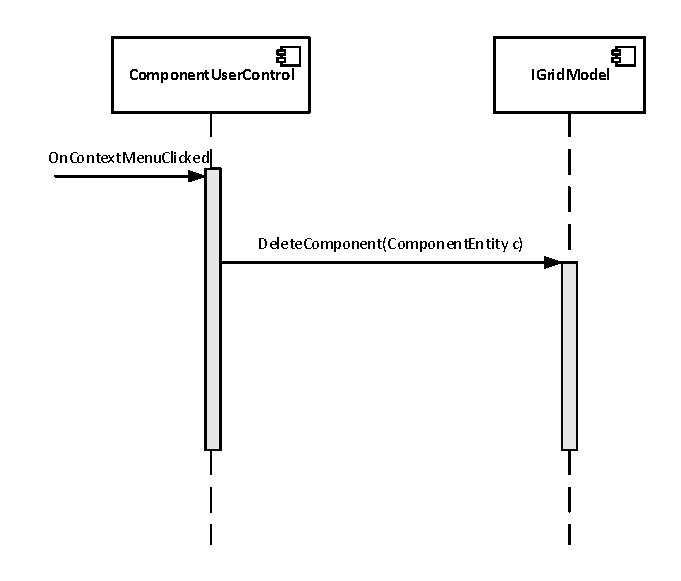
\includegraphics{figures/DeleteComponent}
	\caption{Deleting components.}
\end{figure}

\begin{figure}[!ht]
	\centering
	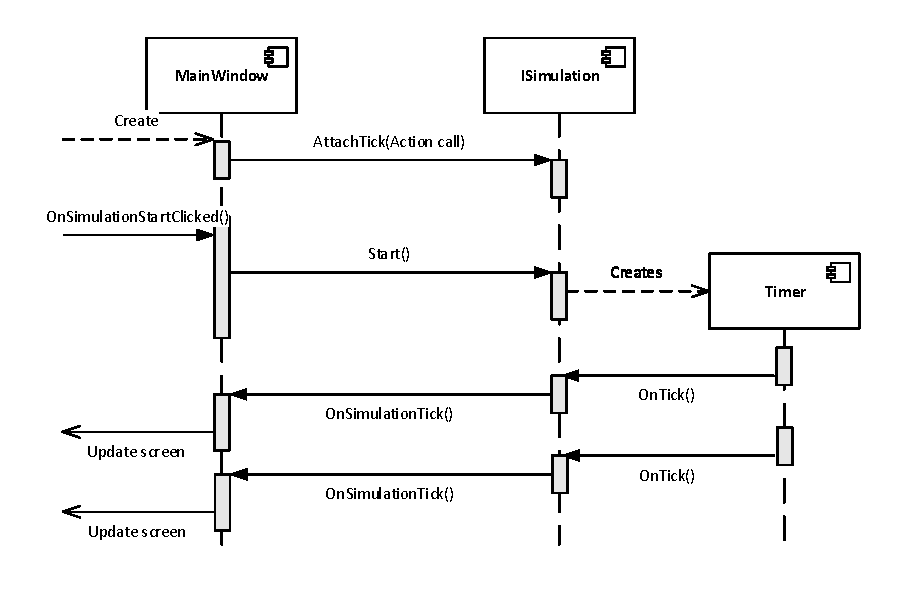
\includegraphics{figures/RunningSimulation}
	\caption{Running simulation.}
\end{figure}

\begin{figure}[!ht]
	\centering
	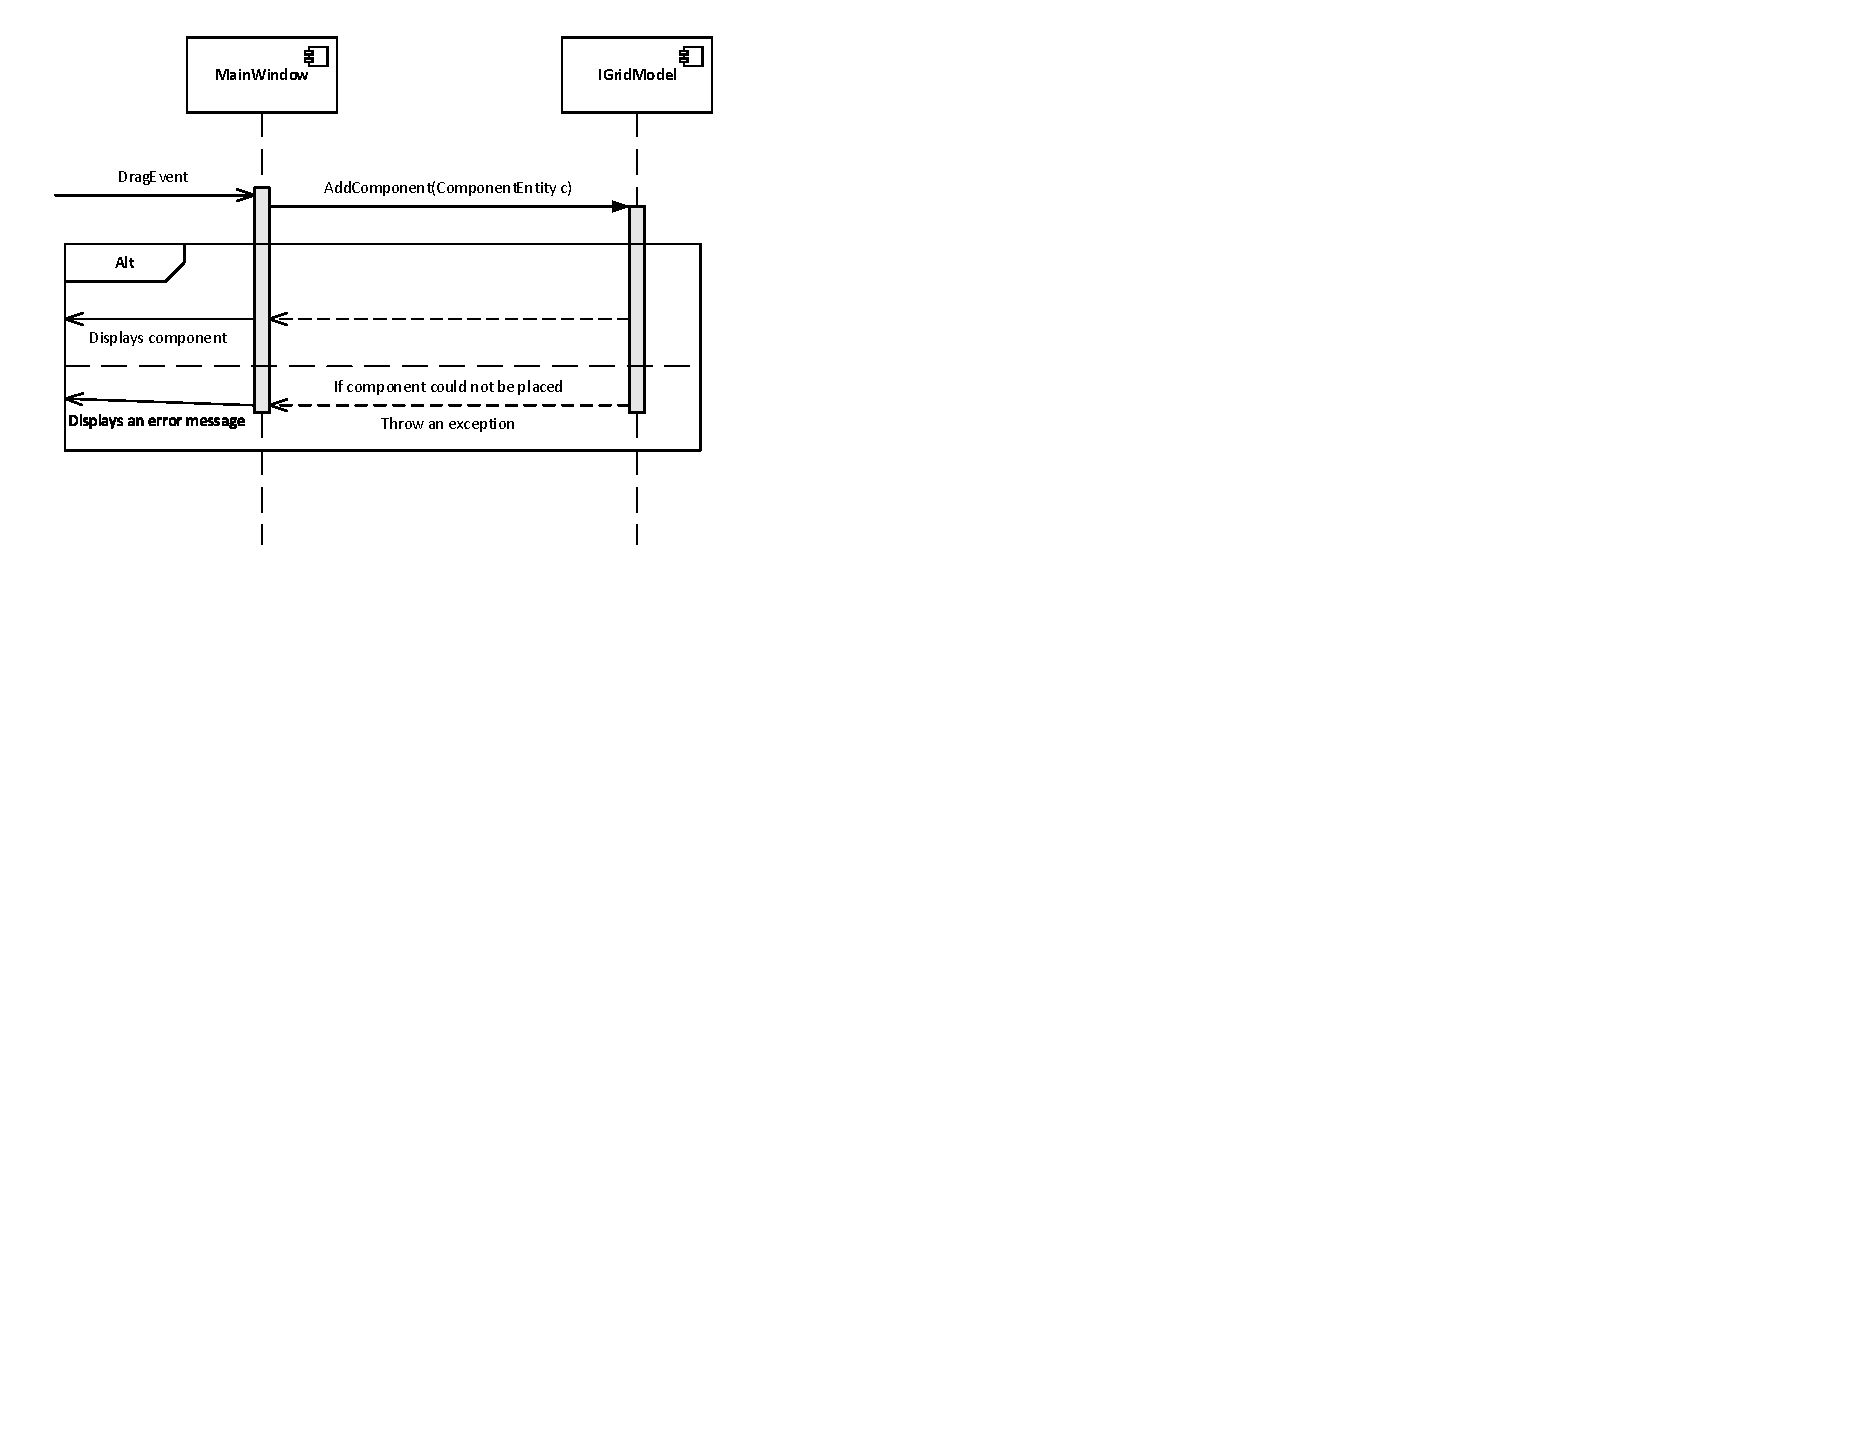
\includegraphics{figures/Stopping}
	\caption{Stopping simulation.}
\end{figure}

\begin{figure}[!ht]
	\centering
	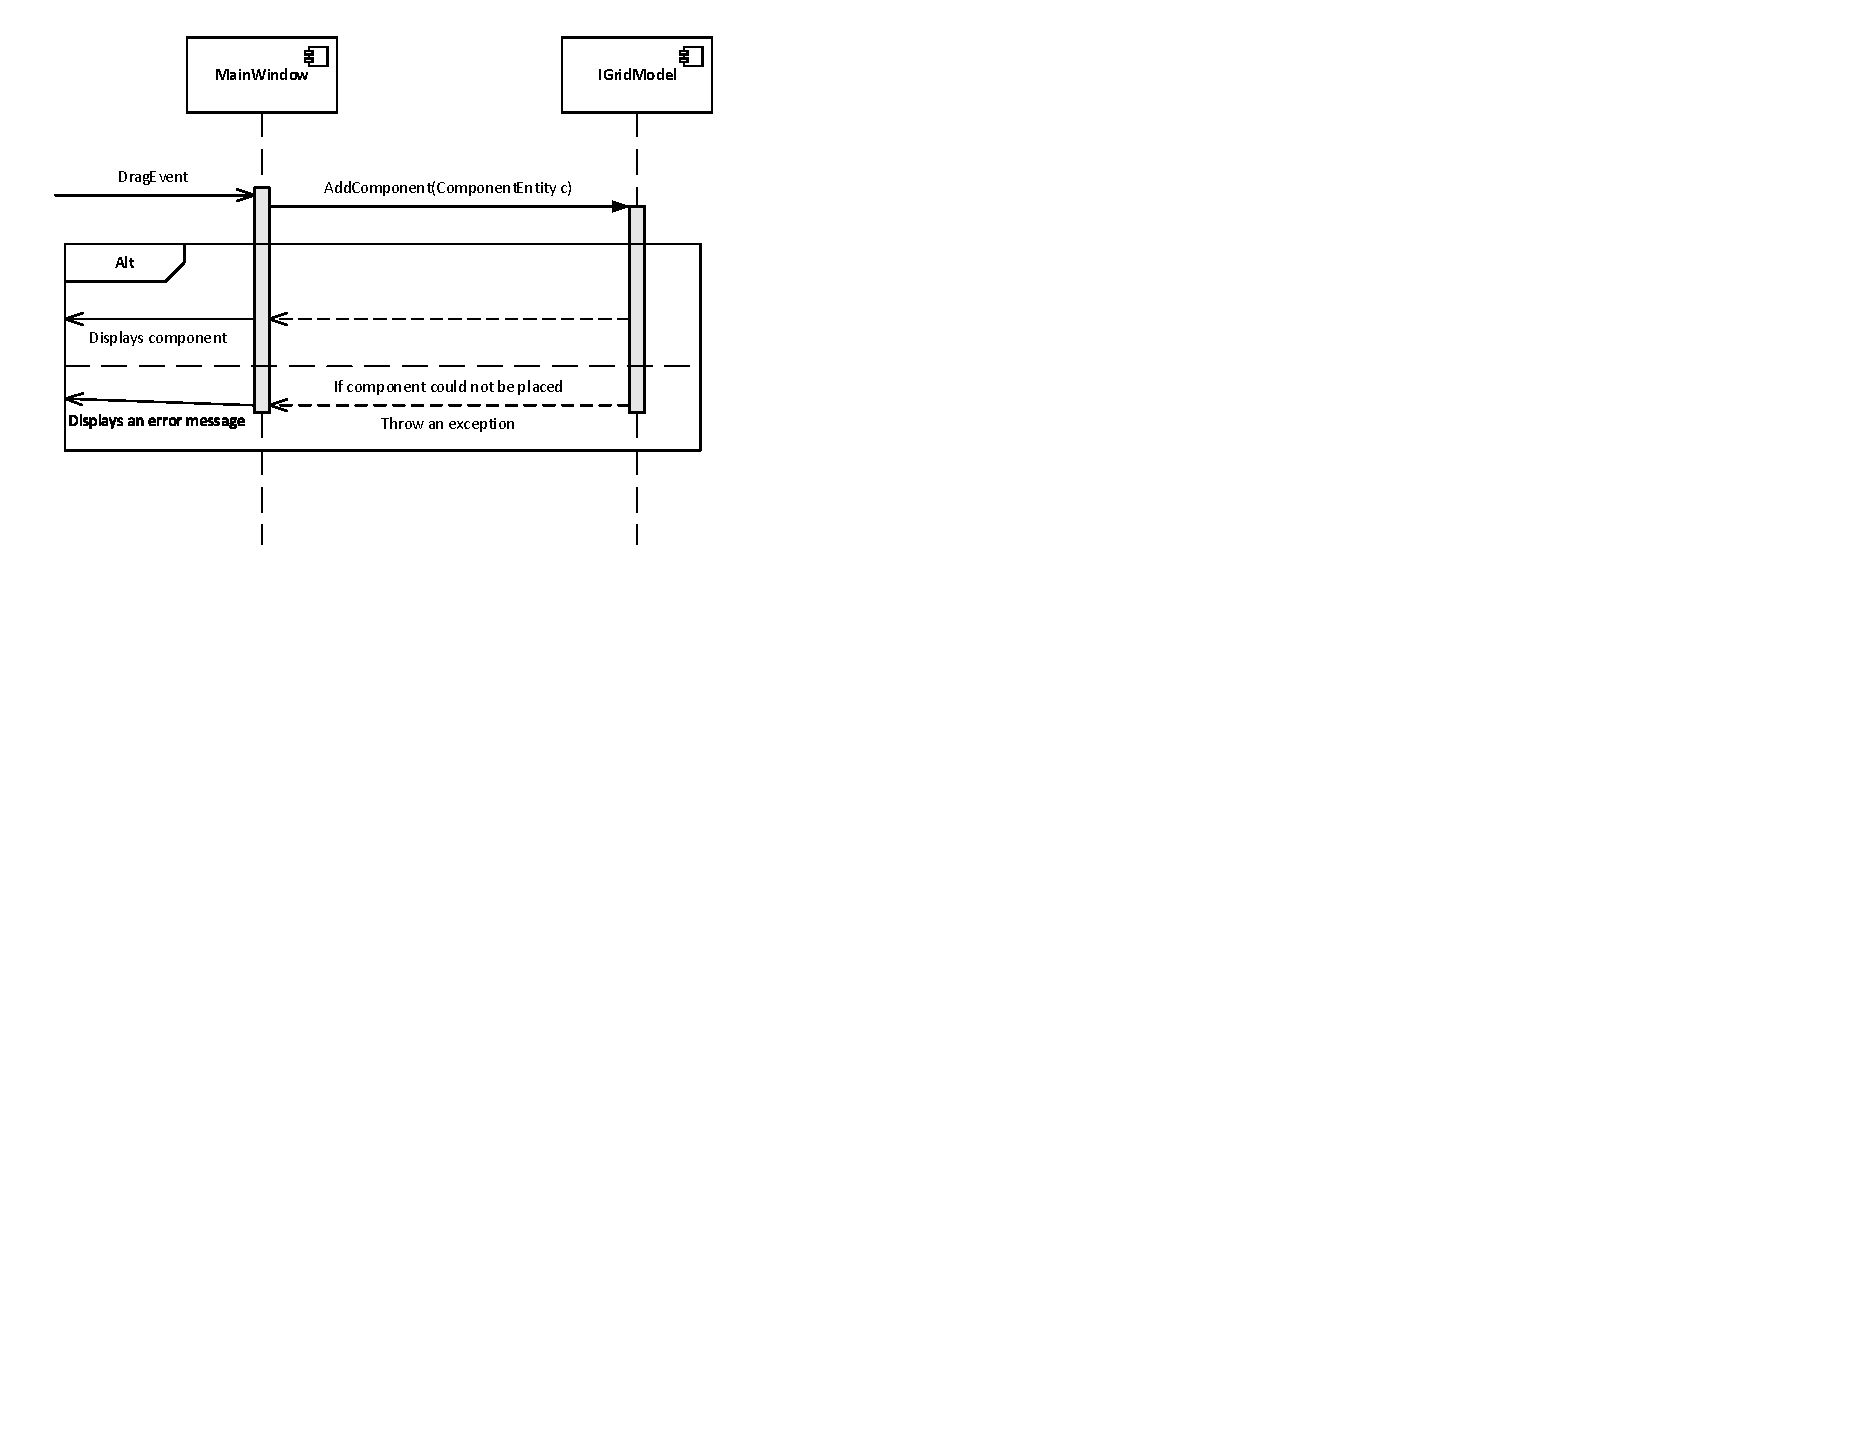
\includegraphics{figures/Pausing}
	\caption{Pausing simulation.}
\end{figure}

\begin{figure}[!ht]
	\centering
	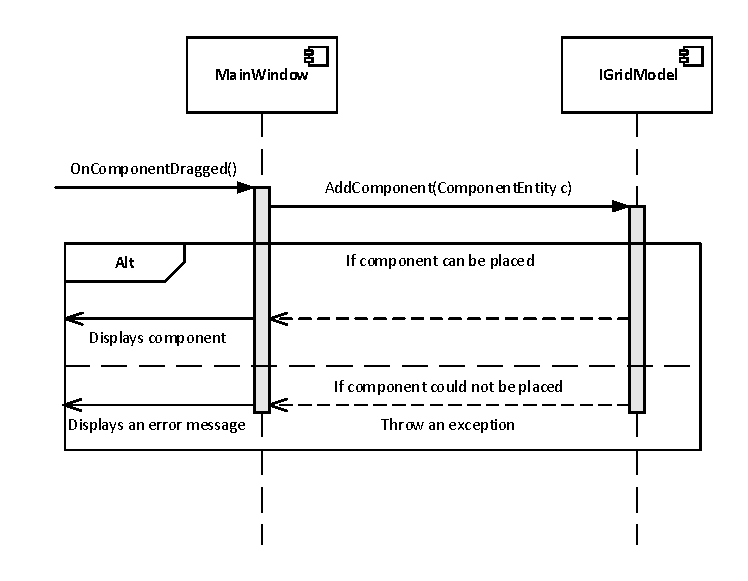
\includegraphics{figures/LoadFile}
	\caption{Opening a file.}
\end{figure}

\begin{figure}[!ht]
	\centering
	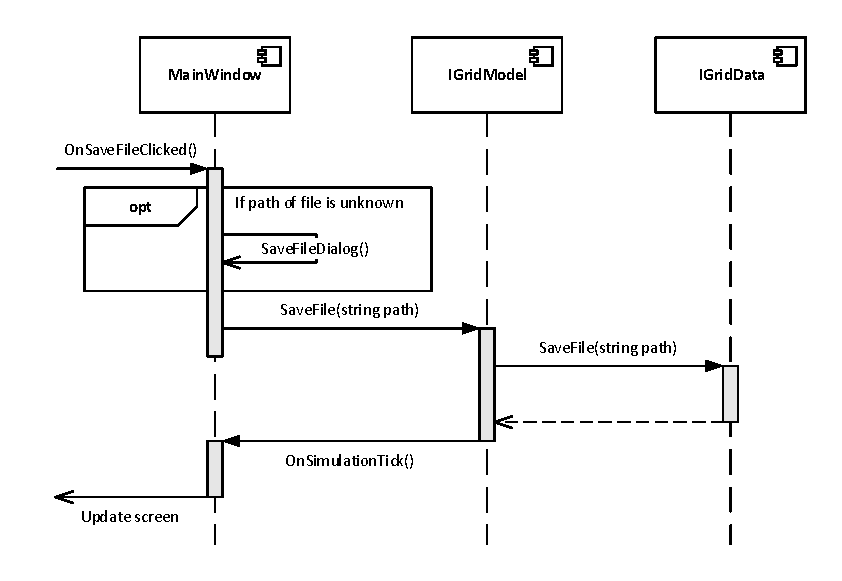
\includegraphics{figures/SaveFile}
	\caption{Saving a file.}
\end{figure}

\begin{figure}[!ht]
	\centering
	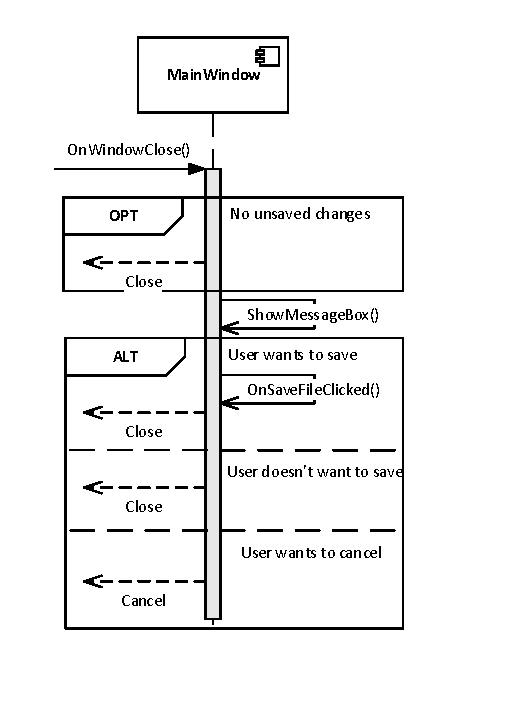
\includegraphics{figures/CloseWindow}
	\caption{Close window.}
\end{figure}
    
    \end{document}